\chapter{Implementasi dan Pengujian}
\label{chap:Implementasi}

Pada bab ini akan ditunjukkan tampilan dari implementasi perangkat lunak dan juga bagaimana perangkat lunak diimplementasikan. Pengujian juga akan diterapkan pada perangkat lunak secara fungsional dan eksperimental. Hasil dari pegujian akan dijelaskan secara rinci dan sistemasi serta akan dibuat kesimpulan untuk pengujian yang telah dilakukan.


% \section{Implementasi Perangkat Lunak}
% \label{sec:implementasi-pl}

% \subsection{Instalasi}
% \label{sec:instalasi}

% \subsection{Antarmuka}
% \label{sec:antarmuka}

% \subsection{Randomisasi}
% \label{sec:randomisasi}


\section{Implementasi Antarmuka}
\label{sec:implementasi-antarmuka}

Antarmuka perangkat lunak diimplementasikan dengan memakai \textit{framework} antarmuka grafis berbasis bahasa pemograman Python yang bernama Kivy\footnote{https://kivy.org/\#home}. Implementasi antarmuka disesuaikan dengan rancangan antarmuka perangkat lunak yang telah dibuat pada bab~\ref{chap:perancangan}. Gambar~\ref{fig:antarmukautama} adalah tampilan antarmuka dari implementasi perangkat lunak.

\begin{figure}
	\centering
	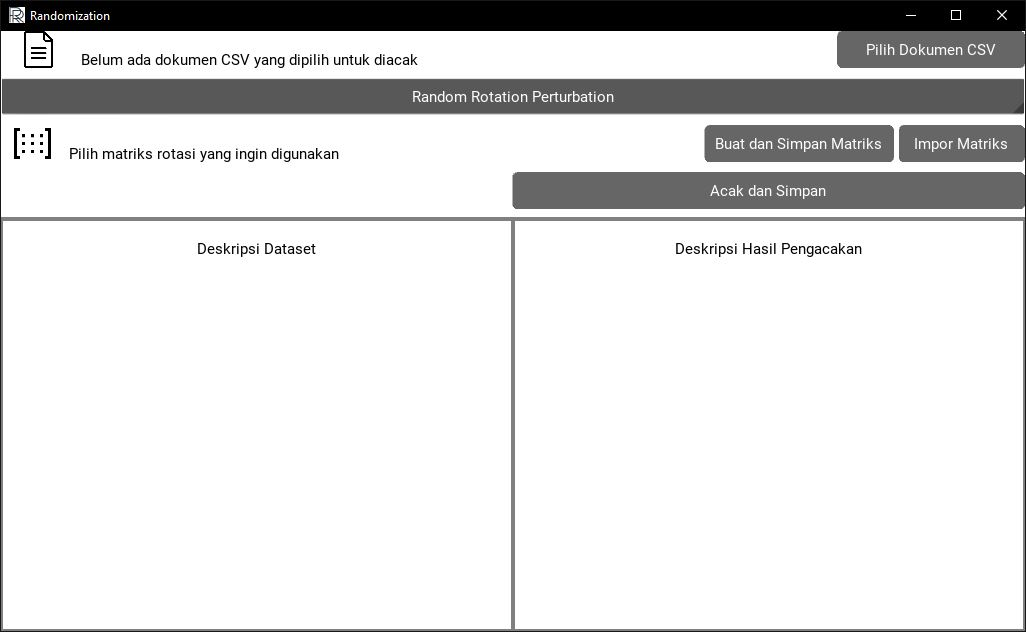
\includegraphics[scale=0.6]{antarmukautama}
	\caption{Tampilan perangkat lunak yang pertama ditampilkan saat perangkat lunak baru dibuka}
	\label{fig:antarmukautama}
\end{figure}

Antarmuka perangkat lunak mempunyai tiga buah bagian yang mempunyai fungsinya masing-masing. Ketiga bagian ini dapat dilihat pada Gambar~\ref{fig:antarmukautamabernomor} Pertama adalah bagian masukan dan pengaturan, terdapat pada bagian atas yang bernomor satu dan dikelilingi kotak merah. Kedua adalah bagian deskripsi dataset, terdapat pada bagian bawah sebelah kiri yang bernomor dua dan dikelilingi kotak biru. Terakhir adalah bagian deskripsi hasil randomisasi, terdapat pada bagian bawah sebelah kanan yang bernomor tiga dan dikelilingi kotak hijau. Ketiga bagian ini akan dijelaskan secara rinci pada subbab-subbab berikutnya.

\begin{figure}
	\centering
	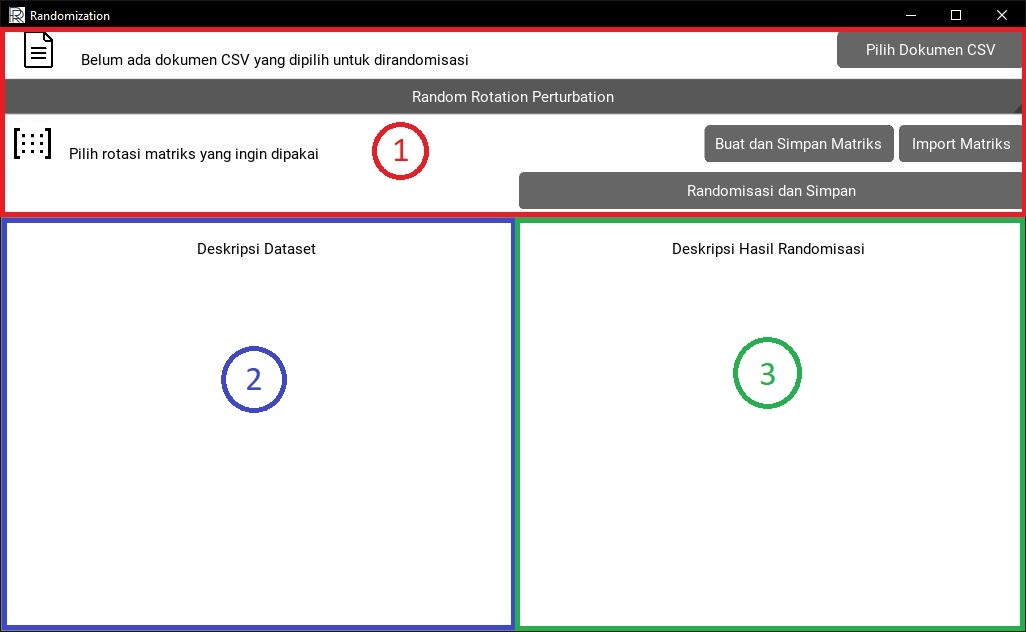
\includegraphics[scale=0.6]{antarmukautamabernomor}
	\caption{Bagian-bagian pada antarmuka perangkat lunak}
	\label{fig:antarmukautamabernomor}
\end{figure}

Perangkat lunak randomisasi ini mengimplementasikan dua buah teknik randomisasi yang berbeda yaitu \textit{Random Rotation Perturbation} dan \textit{Random Projection Perturbation}. Oleh karena itu, antarmuka perangkat lunak akan menyesuaikan dengan teknik yang dipilih oleh pengguna. Ketiga bagian antarmuka yang telah disebutkan tadi dengan otomatis akan berubah sesuai dengan teknik yang dipilih. Pada setiap subbab akan dijelaskan juga sekaligus perbedaan antarmuka teknik randomisasi satu dengan yang lainnya.

\subsection{Masukan dan Pengaturan}
\label{sec:masukanpengaturan}

Bagian masukan dan pengaturan menyediakan berbagai interaksi untuk pengguna dapat mengatur masukan yang perlu diberikan kepada perangkat lunak dan menerapkan teknik randomisasi yang diinginkan. Ada beberapa fungsi inti pada bagian ini yaitu masukan dataset berupa file \textit{comma-separated values} yang ingin dirandomisasi, memilih teknik randomisasi yang ingin digunakan, membuat baru dan memilih matriks rotasi atau proyeksi yang ingin digunakan, masukan nilai variabel \textit{epsilon} dan nilai variabel k untuk teknik \textit{Random Projection Perturbation}, dan sebuah tombol untuk menerapkan teknik randomisasi dan menyimpan hasilnya. Berikut akan dijelaskan secara rinci dengan gambar setiap fungsi tersebut yang dapat dilihat pada Gambar~\ref{fig:antarmukamasukanpengaturan} dan cara pemakaiannya yang benar secara berturut. 

\begin{figure}
	\centering
	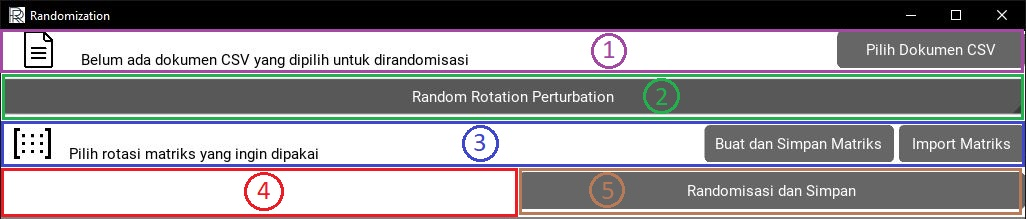
\includegraphics[scale=0.6]{antarmukamasukanpengaturan}
	\caption{Bagian antarmuka masukan dan pengaturan perangkat lunak}
	\label{fig:antarmukamasukanpengaturan}
\end{figure}

\subsubsection{Masukan Dataset}
\label{sec:masukandataset}

Pertama pengguna perlu memberikan masukan dataset yang ingin dirandomisasi berupa dokumen berjenis \textit{comma-separated values}. Perangkat lunak menyediakan fitur tersebut yang dapat dilihat pada Gambar~\ref{fig:antarmukamasukanpengaturan} yang terdapat pada bagian yang dikelilingi kotak berwarna merah bernomor satu. Pengguna dapat menekan tombol "Pilih Dokumen CSV" yang terletak pada ujung sebelah kanan. Tombol ini bertujuan untuk memilih dokumen yang ingin dirandomisasi pada direktori pengguna. Ketika tombol ditekan, perangkat lunak akan membuka jendela baru untuk memilih dokumen yang dapat dilihat pada gambar~\ref{fig:pilihdokumen}.

\begin{figure}
	\centering
	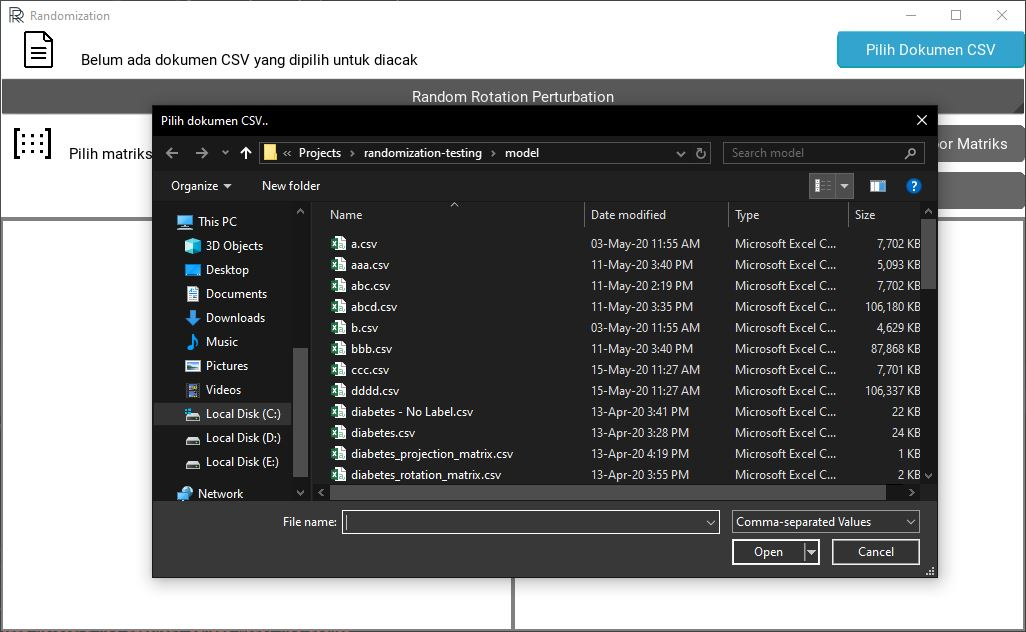
\includegraphics[scale=0.6]{pilihdokumen}
	\caption{Jendela untuk memilih dataset yang berupa dokumen CSV}
	\label{fig:pilihdokumen}
\end{figure}

Setelah pengguna memilih dataset yang diinginkan, perangkat lunak akan otomatis menuliskan lokasi dokumen yang dipilih berada. Perangkat lunak akan menampilkan lokasi dokumen tersebut pada bagian tengah sebelah kanan simbol dokumen dan sebelah kiri tombol "Pilih Dokumen CSV". Jika belum ada dataset yang dipilih maka perangkat lunak akan menampilkan label yang berupa kalimat "Belum ada dokumen CSV yang dipilih untuk dirandomisasi" yang menunjukkan bahwa belum ada dokumen yang dipilih oleh pengguna. Jika pengguna memilih ulang dokumen, maka secara otomatis juga perangkat lunak akan memperbaharui lokasi dokumen sesuai dokumen yang dipilih pengguna.

Apabila dokumen yang dipilih berukuran besar, maka perangkat lunak akan memakan sedikit waktu yang lebih lama. Dalam rangka memberitahukan kepada pengguna bahwa perangkat lunak sedang melakukan proses pemilihan dokumen, perangkat lunak akan menampilkan sebuah \textit{popup} yang memberitahukan bahwa proses pemilihan sedang berjalan dan perangkat lunak tidak berhenti bekerja maupun \textit{error} sehingga pengguna tidak bingung apabila perangkat lunak memakan waktu yang lebih lama untuk memproses dokumen yang dipilih. Tampilan antarmuka \textit{popup} tersebut dapat dilihat pada Gambar~\ref{fig:loadingmemilihdokumen}. Setelah dokumen dipilih pengguna dan perangkat lunak berhasil memproses dokumen tersebut, perangkat lunak akan memperbaharui lokasi dokumen dan menampilkan beberapa informasi dataset yang dipilih pada bagian deskripsi dataset yang akan dijelaskan pada subbab berikutnya. Tampilan antarmuka setelah pengguna memilih dokumen dapat dilihat pada Gambar~\ref{fig:dokumendipilih}

\begin{figure}
	\centering
	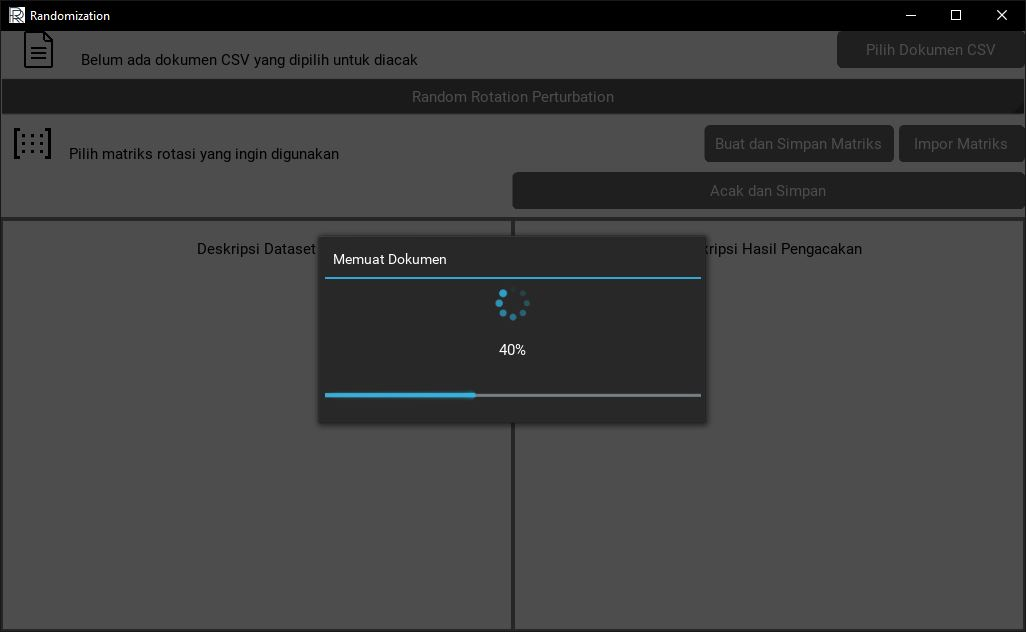
\includegraphics[scale=0.6]{loadingmemilihdokumen}
	\caption{Tampilan \textit{popup} yang muncul saat proses berlangsung}
	\label{fig:loadingmemilihdokumen}
\end{figure}

\begin{figure}
	\centering
	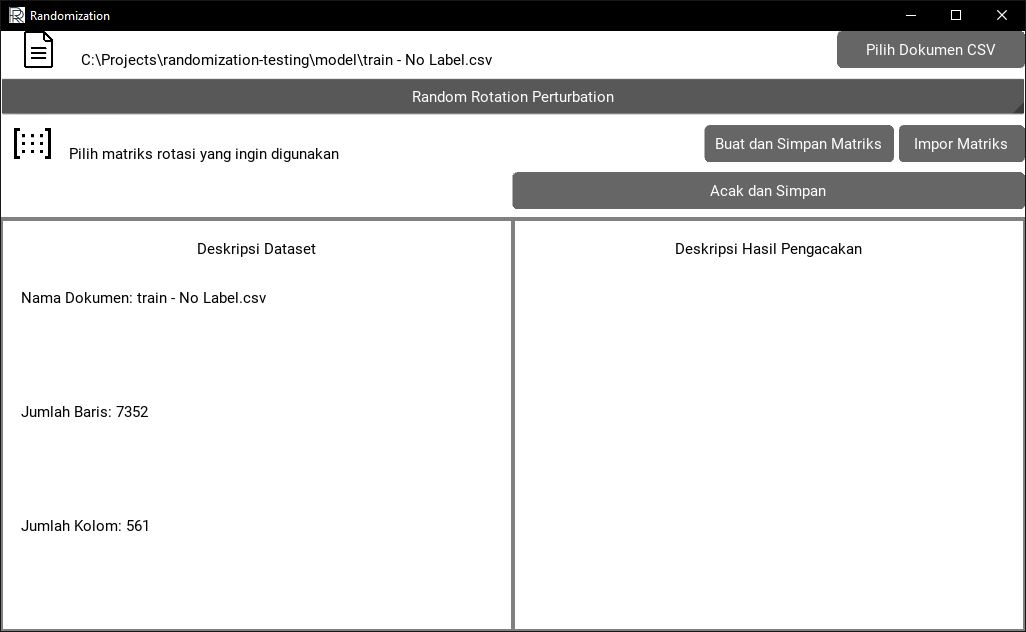
\includegraphics[scale=0.6]{dokumendipilih}
	\caption{Tampilan antarmuka setelah sebuah dokumen dipilih}
	\label{fig:dokumendipilih}
\end{figure}

Selain itu setelah pengguna memilih dokumen CSV, perangkat lunak akan membaca dokumen tersebut dan memproses isi dari dokumen tersebut menjadi dataset yang berupa matriks. Proses ini dilakukan sekali saja tepat setelah pengguna memilih dokumen dengan menekan tombol "Pilih Dokumen CSV". Oleh karena itu, apabila sebuah dokumen CSV diubah isinya setelah dokumen tersebut dipilih oleh pengguna maka perangkat lunak tetap akan menggunakan isi dari dokumen tersebut yang belum diubah. Pengguna harus berhati-hati apabila isi dokumen diubah maka pengguna juga harus memilih kembali dokumen yang sama tersebut walaupun perangkat lunak sudah menunjukkan lokasi dokumen yang digunakan adalah dokumen yang pengguna inginkan.

\subsubsection{Pemilihan Teknik Randomisasi}
\label{sec:pilihteknik}

Setelah pengguna memilih dataset yang ingin dirandomisasi, pengguna juga harus memilih teknik randomisasi apa yang ingin diterapkan terhadap dataset yang sudah dipilih. Pada awal perangkat lunak dibuka, secara otomatis teknik \textit{Random Rotation Perturbation} yang dipilih. Apabila pengguna ingin mengganti teknik yang ingin diterapkan pada dataset, pengguna dapat menekan tombol \textit{dropdown} yang bertuliskan nama teknik randomisasi. Tombol ini dapat dilihat pada Gambar~\ref{fig:antarmukamasukanpengaturan} yang dikelilingi kotak berwarna hijau dan bernomor 2.

Apabila pengguna menekan tombol ini maka perangkat lunak akan menampilkan \textit{dropdown} yang mempunyai dua buah opsi teknik randomisasi yaitu "Random Rotation Perturbation" dan "Random Projection Perturbation". Antarmuka tersebut dapat dilihat pada Gambar~\ref{fig:opsipilihteknik} yang dikelilingi oleh kotak merah. Pemilihan teknik ini juga akan memicu beberapa perubahan pada tampilan antarmuka perangkat lunak menyesuaikan dengan teknik yang dipilih. Beberapa perubahan pada perangkat lunak tersebut melingkupi bagian pembuatan dan pemilihan matriks, parameter teknik randomisasi, dan bagian randomisasi dan simpan yang akan dijelaskan setiap perubahan tersebut pada subbab berikutnya.

\begin{figure}
	\centering
	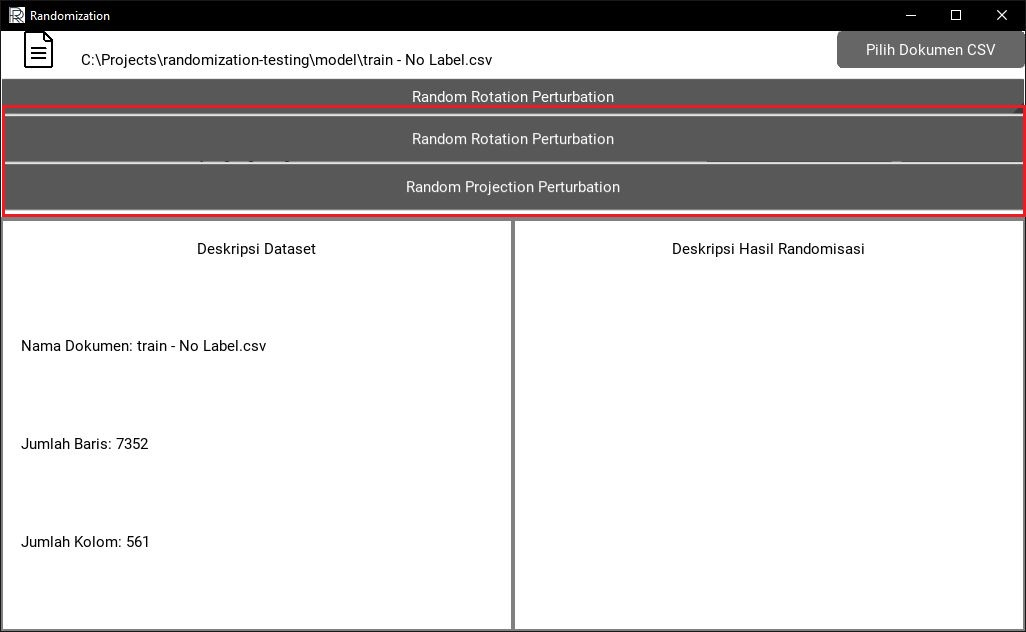
\includegraphics[scale=0.6]{opsipilihteknik}
	\caption{Tampilan antarmuka setelah sebuah dokumen dipilih}
	\label{fig:opsipilihteknik}
\end{figure}

\subsubsection{Pembuatan dan Pemilihan Matriks}
\label{sec:pilihmatriks}

Setelah pengguna memilih teknik yang ingin diterapkan, pengguna harus memilih matriks yang diinginkan atau membuat baru. Matriks yang dimaksudkan adalah matriks rotasi atau matriks proyeksi sesuai teknik randomisasi yang dipilih. Apabila teknik \textit{Random Rotation Perturbation} yang dipilih maka perangkat lunak akan mengubah fungsi pembuatan dan pemilihan matriks ini menjadi matriks rotasi. Apabila teknik \textit{Random Projection Perturbation} yang dipilih maka perangkat lunak akan mengubah fungsi pembuatan dan pemilihan matriks ini menjadi matriks proyeksi. Perubahan ini dapat terlihat pada label yang berada di sebelah kanan simbol matriks apabila belum memilih atau membuat matriks maka label tersebut akan menampilkan kalimat "Pilih matriks rotasi yang ingin digunakan" atau "Pilih matriks proyeksi yang ingin digunakan".

Ada dua buah tombol pada bagian ini yaitu "Buat dan Simpan Matriks" dan "Import Matriks". Tombol "Buat dan Simpan Matriks" mempunyai fungsi untuk membuat matriks rotasi atau proyeksi baru sesuai teknik randomisasi yang dipilih dan menyimpan matriks tersebut pada sebuah dokumen CSV baru yang dibuat oleh perangkat lunak pada direktori tertentu yang akan dipilih oleh pengguna. Hasil matriks yang dibuat oleh perangkat lunak dapat digunakan kembali untuk lain kali sehingga rotasi atau proyeksi yang diterapkan akan sama dengan yang sebelumnya. Pengguna dapat melakukan ini dengan cara menekan tombol "Import Matriks" untuk memilih matriks rotasi atau proyeksi yang diinginkan untuk diterapkan pada dataset. Matriks yang dipilih harus sesuai dengan dataset yang ingin dirandomisasi, misalnya apabila matriks rotasi yang dipilih memiliki dimensi yang berbeda dengan dataset maka perangkat lunak akan melarang impor matriks dilakukan karena randomisasi tidak dapat dilakukan.

\subsubsection{Parameter Teknik Randomisasi}
\label{sec:parameterteknik}

\subsubsection{Randomisasi dan Simpan}
\label{sec:randomisasisimpan}


\subsection{Deskripsi Dataset}
\label{sec:deskripsidataset}

\subsection{Deskripsi Hasil Randomisasi}
\label{sec:masukanpengaturan}



\section{Pengujian Perangkat Lunak}
\label{sec:pengujianpl}

\subsection{Pengujian Fungsional}
\label{sec:pengujianfungsional}

\subsection{Pengujian Eksperimental}
\label{sec:pengujianeksperimental}